% Options for packages loaded elsewhere
\PassOptionsToPackage{unicode}{hyperref}
\PassOptionsToPackage{hyphens}{url}
%
\documentclass[
  ignorenonframetext,
]{beamer}
\title{Comments on Das}
\author{Brian Weatherson}
\date{January 2022}

\usepackage{pgfpages}
\setbeamertemplate{caption}[numbered]
\setbeamertemplate{caption label separator}{: }
\setbeamercolor{caption name}{fg=normal text.fg}
\beamertemplatenavigationsymbolsempty
% Prevent slide breaks in the middle of a paragraph
\widowpenalties 1 10000
\raggedbottom
\setbeamertemplate{part page}{
  \centering
  \begin{beamercolorbox}[sep=16pt,center]{part title}
    \usebeamerfont{part title}\insertpart\par
  \end{beamercolorbox}
}
\setbeamertemplate{section page}{
  \centering
  \begin{beamercolorbox}[sep=12pt,center]{part title}
    \usebeamerfont{section title}\insertsection\par
  \end{beamercolorbox}
}
\setbeamertemplate{subsection page}{
  \centering
  \begin{beamercolorbox}[sep=8pt,center]{part title}
    \usebeamerfont{subsection title}\insertsubsection\par
  \end{beamercolorbox}
}
\AtBeginPart{
  \frame{\partpage}
}
\AtBeginSection{
  \ifbibliography
  \else
    \frame{\sectionpage}
  \fi
}
\AtBeginSubsection{
  \frame{\subsectionpage}
}
\usepackage{amsmath,amssymb}
\usepackage{lmodern}
\usepackage{iftex}
\ifPDFTeX
  \usepackage[T1]{fontenc}
  \usepackage[utf8]{inputenc}
  \usepackage{textcomp} % provide euro and other symbols
\else % if luatex or xetex
  \usepackage{unicode-math}
  \defaultfontfeatures{Scale=MatchLowercase}
  \defaultfontfeatures[\rmfamily]{Ligatures=TeX,Scale=1}
  \setmainfont[BoldFont = SF Pro Rounded Semibold]{SF Pro Rounded}
  \setmathfont[]{Fira Math}
\fi
\usefonttheme{serif}
\usefonttheme{serif} % use mainfont rather than sansfont for slide text
% Use upquote if available, for straight quotes in verbatim environments
\IfFileExists{upquote.sty}{\usepackage{upquote}}{}
\IfFileExists{microtype.sty}{% use microtype if available
  \usepackage[]{microtype}
  \UseMicrotypeSet[protrusion]{basicmath} % disable protrusion for tt fonts
}{}
\makeatletter
\@ifundefined{KOMAClassName}{% if non-KOMA class
  \IfFileExists{parskip.sty}{%
    \usepackage{parskip}
  }{% else
    \setlength{\parindent}{0pt}
    \setlength{\parskip}{6pt plus 2pt minus 1pt}}
}{% if KOMA class
  \KOMAoptions{parskip=half}}
\makeatother
\usepackage{xcolor}
\IfFileExists{xurl.sty}{\usepackage{xurl}}{} % add URL line breaks if available
\IfFileExists{bookmark.sty}{\usepackage{bookmark}}{\usepackage{hyperref}}
\hypersetup{
  pdftitle={Comments on Das},
  pdfauthor={Brian Weatherson},
  hidelinks,
  pdfcreator={LaTeX via pandoc}}
\urlstyle{same} % disable monospaced font for URLs
\newif\ifbibliography
\usepackage{longtable,booktabs,array}
\usepackage{calc} % for calculating minipage widths
\usepackage{caption}
% Make caption package work with longtable
\makeatletter
\def\fnum@table{\tablename~\thetable}
\makeatother
\usepackage{graphicx}
\makeatletter
\def\maxwidth{\ifdim\Gin@nat@width>\linewidth\linewidth\else\Gin@nat@width\fi}
\def\maxheight{\ifdim\Gin@nat@height>\textheight\textheight\else\Gin@nat@height\fi}
\makeatother
% Scale images if necessary, so that they will not overflow the page
% margins by default, and it is still possible to overwrite the defaults
% using explicit options in \includegraphics[width, height, ...]{}
\setkeys{Gin}{width=\maxwidth,height=\maxheight,keepaspectratio}
% Set default figure placement to htbp
\makeatletter
\def\fps@figure{htbp}
\makeatother
\setlength{\emergencystretch}{3em} % prevent overfull lines
\providecommand{\tightlist}{%
  \setlength{\itemsep}{0pt}\setlength{\parskip}{0pt}}
\setcounter{secnumdepth}{-\maxdimen} % remove section numbering
\let\Tiny=\tiny

 \setbeamertemplate{navigation symbols}{} 

% \usetheme{Madrid}
 \usetheme[numbering=none, progressbar=foot]{metropolis}
 \usecolortheme{wolverine}
 \usepackage{color}
 \usepackage{MnSymbol}
% \usepackage{movie15}

\usepackage{amssymb}% http://ctan.org/pkg/amssymb
\usepackage{pifont}% http://ctan.org/pkg/pifont
\newcommand{\cmark}{\ding{51}}%
\newcommand{\xmark}{\ding{55}}%

\usepackage{tabulary}

\setlength{\parskip}{1ex plus 0.5ex minus 0.2ex}

\AtBeginSection[]
{
\begin{frame}
	\Huge{\color{darkblue} \insertsection}
\end{frame}
}

\renewenvironment*{quote}	
	{\list{}{\rightmargin   \leftmargin} \item } 	
	{\endlist }


\usepackage{caption}
\captionsetup[figure]{labelformat=empty}
\ifLuaTeX
  \usepackage{selnolig}  % disable illegal ligatures
\fi

\begin{document}
\frame{\titlepage}

\begin{frame}[b]{Bibliographic Note}
\protect\hypertarget{bibliographic-note}{}
~

\begin{figure}
\centering
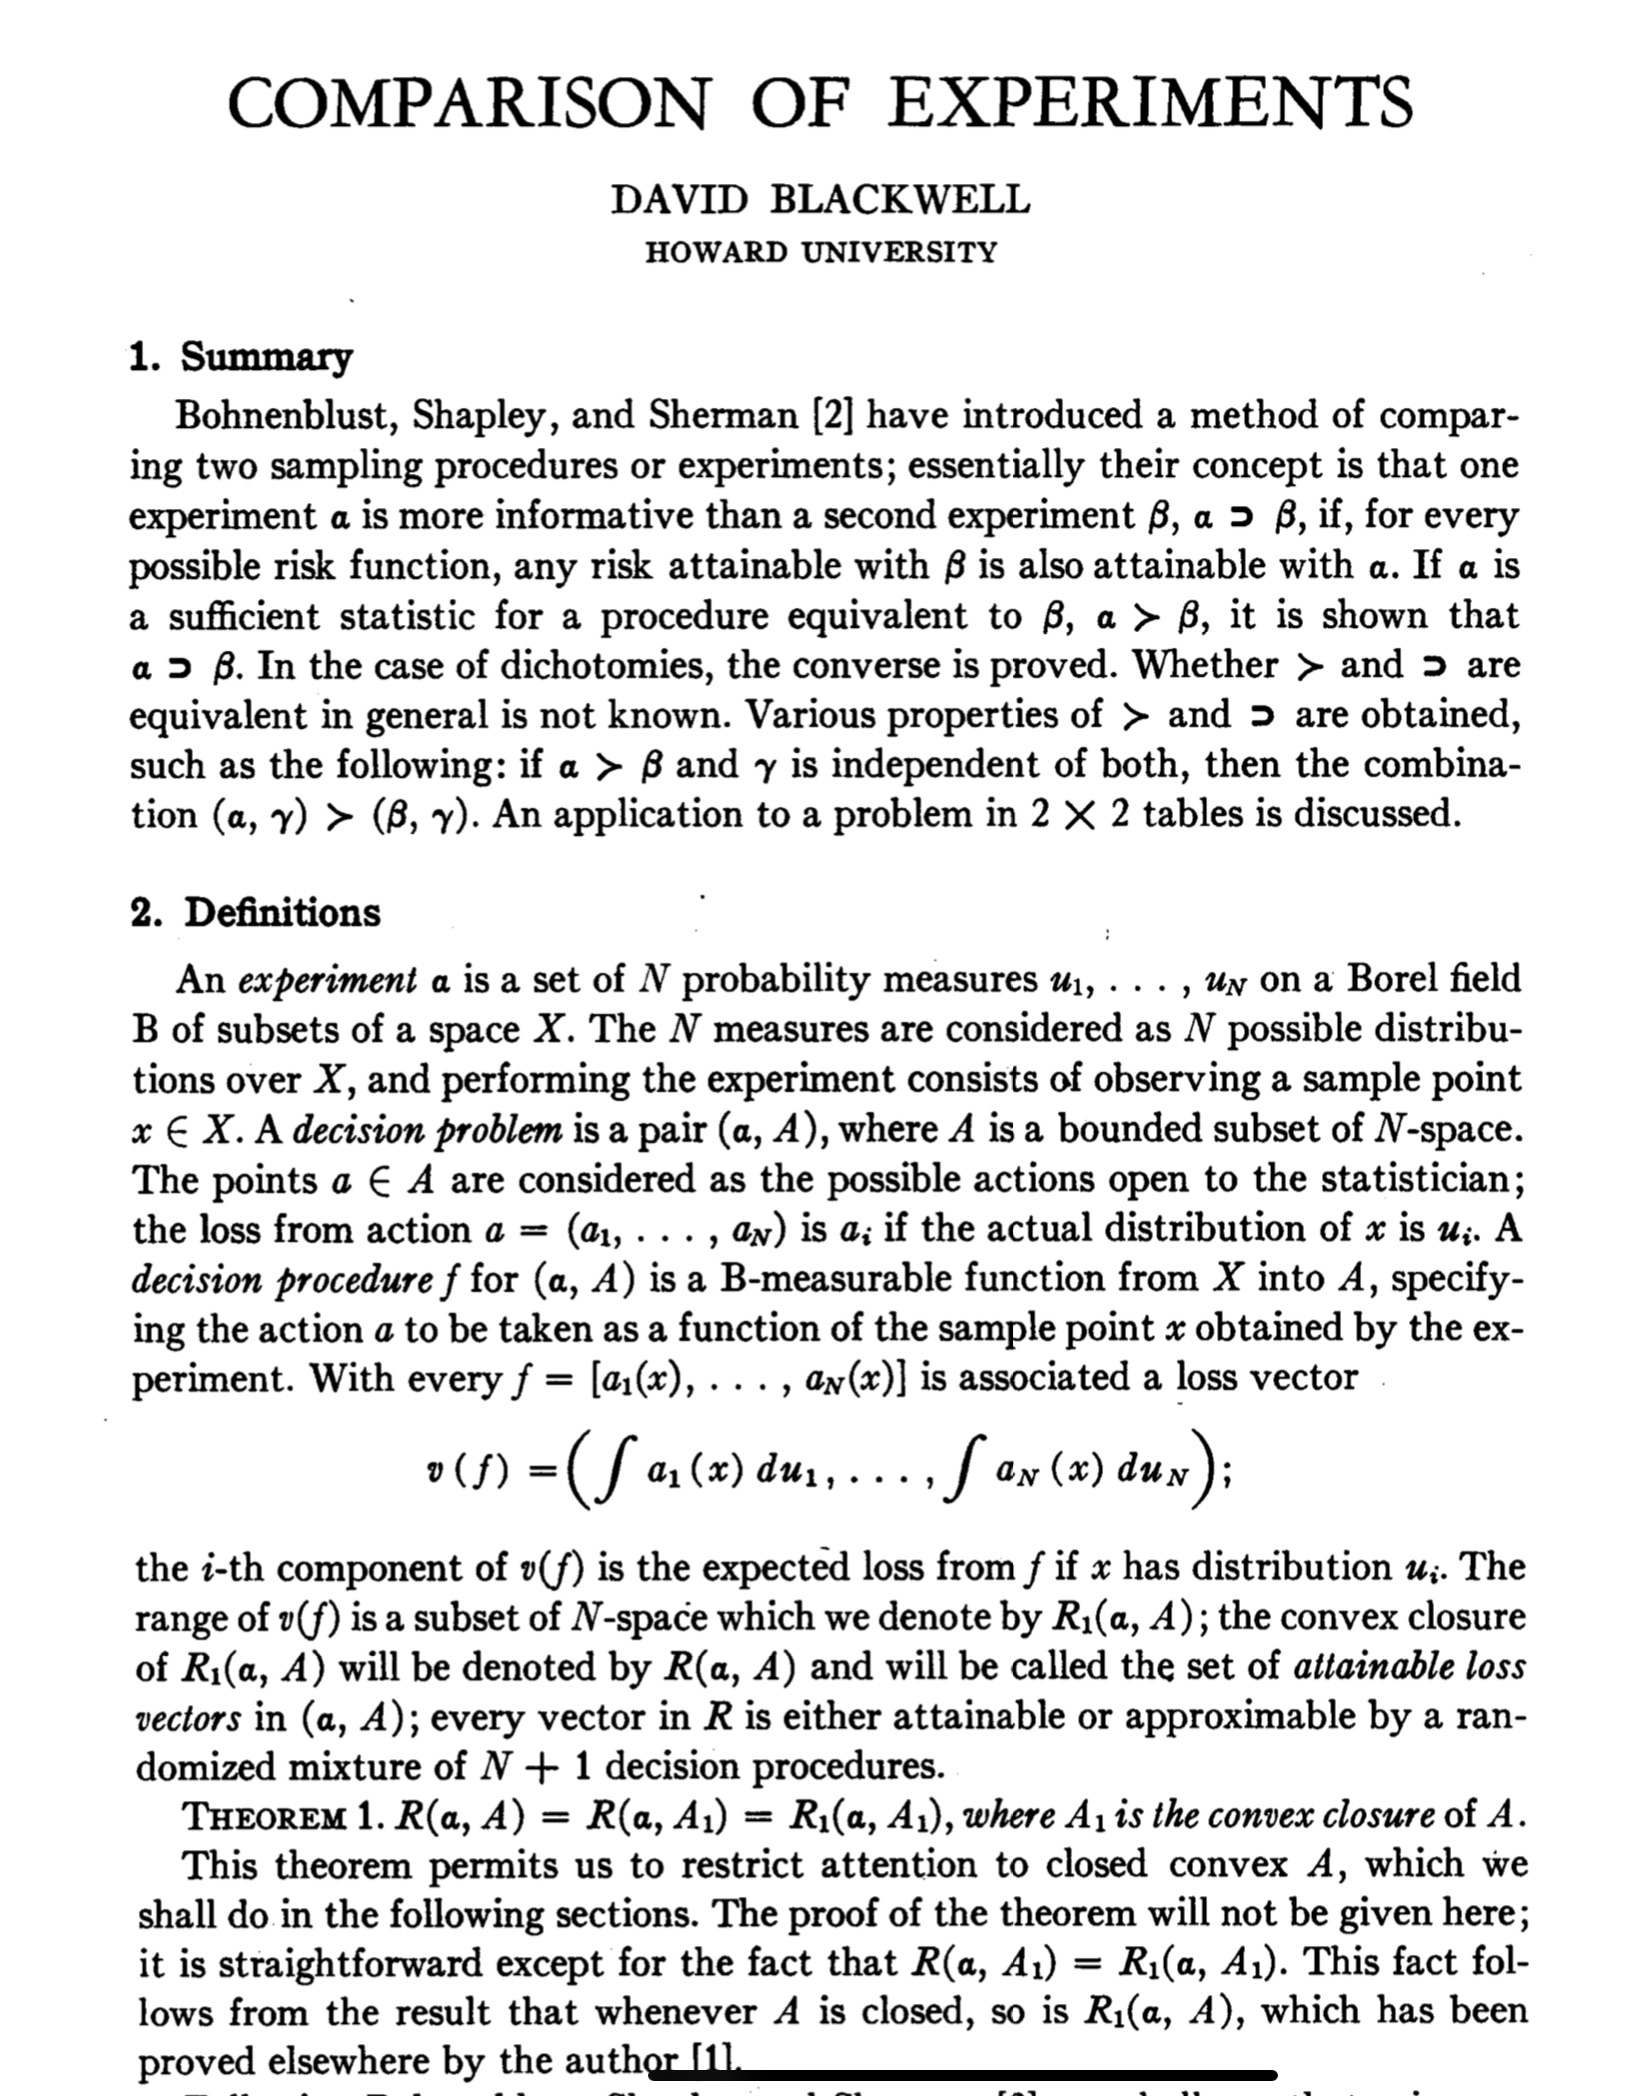
\includegraphics[width=\textwidth,height=0.7\textheight]{blackwell.png}
\caption{David Blackwell, ``Comparison of Experiments'', Berkeley
Symposium on Mathematical Statistics and Probability, 1951}
\end{figure}
\end{frame}

\begin{frame}{Two Questions}
\protect\hypertarget{two-questions}{}
\begin{enumerate}
\tightlist
\item
  Is the value of evidence thesis true?
\item
  Is Nilanjan's decision rule good?
\end{enumerate}
\end{frame}

\begin{frame}{Counterexamples to Value of Evidence}
\protect\hypertarget{counterexamples-to-value-of-evidence}{}
\begin{itemize}[<+->]
\tightlist
\item
  When others know what kind of knowledge you have.
\item
  When knowledge affects value, e.g., spoilers.
\item
  When knowledge comes to a group.
\end{itemize}
\end{frame}

\begin{frame}{A Group Example}
\protect\hypertarget{a-group-example}{}
The group has to choose between these three options.

\begin{longtable}[]{@{}lcc@{}}
\toprule
& p & \textasciitilde p \\
\midrule
\endhead
A & 10 & 0 \\
B & 0 & 10 \\
C & 4 & 4 \\
\bottomrule
\end{longtable}
\end{frame}

\begin{frame}{One Decision Rule}
\protect\hypertarget{one-decision-rule}{}
\begin{itemize}[<+->]
\tightlist
\item
  We do whatever choice maximises the minimum expected utility across
  the group.
\item
  We will do C whatever evidence comes in, but no one wants that either
  now or later.
\item
  In fact everyone would pay 1 to avoid that outcome.
\end{itemize}
\end{frame}

\begin{frame}{Other Decision Rules}
\protect\hypertarget{other-decision-rules}{}
\begin{itemize}
\tightlist
\item
  Let's try dictatorship.
\item
  There might be an Arrovian argument that we'll be forced into
  dictatorship.
\item
  Very hard to get a decision rule that is Paretian and Blackwellian
  other than dictatorship. (Does hard mean impossible? Good question -
  if someone wants to work this out/write this up, lmk.)
\end{itemize}
\end{frame}

\begin{frame}{But It's a Good Dictatorship, Right}
\protect\hypertarget{but-its-a-good-dictatorship-right}{}
~

\begin{figure}
\centering
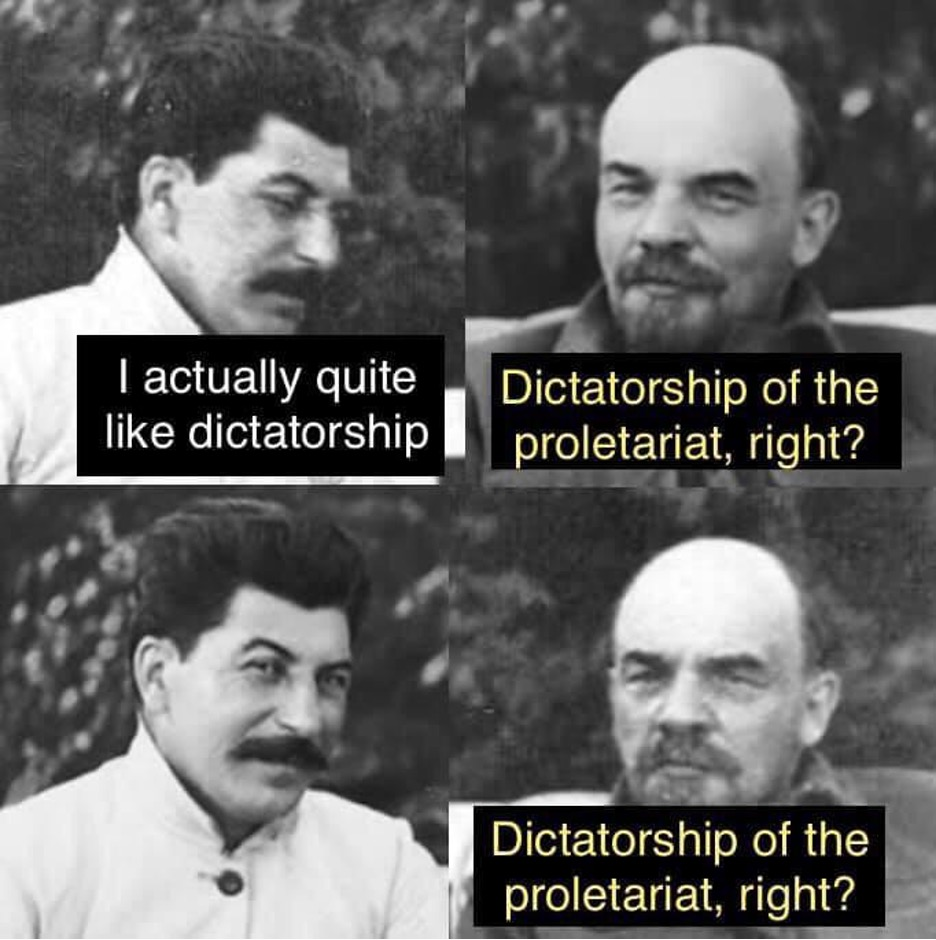
\includegraphics[width=\textwidth,height=0.7\textheight]{dictatorship.jpg}
\caption{From qatsimai on the reddit forum historymemes}
\end{figure}
\end{frame}

\begin{frame}{Nilanjan and the Dictators}
\protect\hypertarget{nilanjan-and-the-dictators}{}
\begin{itemize}
\tightlist
\item
  One of the Pr on the credal committee gets to call the shots.
\item
  This avoids incoherence, as long as the dictator is coherent.
\end{itemize}
\end{frame}

\begin{frame}{Functionalist Worries}
\protect\hypertarget{functionalist-worries}{}
\begin{itemize}
\tightlist
\item
  What does it mean to say other Pr are even in the committee?
\end{itemize}
\end{frame}

\begin{frame}{Am I Really on the Committee?}
\protect\hypertarget{am-i-really-on-the-committee}{}
~

\begin{figure}
\centering

\includegraphics[width=\textwidth,height=0.7\textheight]{missing.jpg}
\caption{The dictator on the credal committee}
\end{figure}
\end{frame}

\begin{frame}{Inquiry}
\protect\hypertarget{inquiry}{}
\begin{itemize}[<+->]
\tightlist
\item
  The solution is to say that the dictator only stays in the job for the
  length of an inquiry, then there is a new lottery.
\item
  But some inquiries run for decades.
\end{itemize}
\end{frame}

\begin{frame}{Suggestion One: Politics are Everywhere}
\protect\hypertarget{suggestion-one-politics-are-everywhere}{}
\begin{itemize}
\tightlist
\item
  The credal committee is a committee, and how it chooses is a political
  problem.
\item
  Live with evidence being costly.
\item
  We're used to that in committee choices already.
\end{itemize}
\end{frame}

\begin{frame}{Suggestion Two: Irrationality is Everywhere}
\protect\hypertarget{suggestion-two-irrationality-is-everywhere}{}
\begin{itemize}
\tightlist
\item
  Does each committee member regard the others as rational, assuming
  known conditionalisation?
\item
  They regard the others as being procedurally rational, but perhaps not
  substantively rational.
\item
  Each other is rational by the other's lights, but not by mine.
\item
  So maybe I shouldn't be surprised that I want to keep information from
  them.
\end{itemize}
\end{frame}

\begin{frame}
~

\begin{figure}
\centering

\includegraphics[width=\textwidth,height=0.9\textheight]{thumbs-cats.jpg}
\caption{~}
\end{figure}
\end{frame}

\end{document}
